\chapter{Hidden Markov Models}
Many of the techniques we've considered so far in this book have been motivated by the \textit{types} of data we could expect to work with. For example, the supervised learning techniques (forms of regression, neural networks, support vector machines, etc.) were motivated by the fact that we had labelled training data. We ventured into clustering to group unlabelled data and discussed dimensionality reduction to handle overly high-dimensional data. In the previous chapter, we examined techniques for managing \textit{incomplete} data with latent variable models. In this chapter we turn to a technique for handling data indexed by \textit{time}.

\section{Motivation}
One major type of data we have not yet paid explicit attention to is \textit{time series} data. Most of the information we record comes with some sort of a timestamp. For example, any time we take an action online, there is a high probability that the database storing that data also tracks it with a timestamp. Physical sensors in the real world always record timestamps because it would be very difficult to make sense of their information if it is not indexed by time. When we undergo medical exams, the results are recorded along with a timestamp. It's almost inconceivable at this point that we would record information without also keeping track of when that data was generated, or at the very least when we saved that data.

There are a variety of reasons to treat time as a special type of data. As we've already discussed, it's a near-universal feature because we so frequently record timestamp information. It's difficult to imagine a data set that couldn't come with timestamps attached to the individual data points. Time also encodes a lot of information that we take for granted about the physical and digital worlds. For example, if the sensors on a plane record the position of the plane at a specific point in time, we would expect the surrounding data points to be relatively similar, or at least move in a consistent direction. In a more general sense, we expect that time constrains other aspects of the data it is attached to in specific ways.

Because we know time posseses these unique properties, it follows that we should exploit them to create more expressive models. In this chapter, we will focus on one such model known as a \textbf{Hidden Markov Model} or \textbf{HMM}. At a high level, the goal of an HMM is to model the state of an entity over time, with the caveat that we never actually observe the state itself. Instead, we observe a data point $\textbf{x}_t$ at each time step (often called an `emission') that is some function of the true state $\textbf{s}_t$. For example, we could model the position of a robot over time given a noisy estimation of the robot's current position at each time step. Furthermore, we have some belief about how one state $\textbf{s}_t$ transitions to the next state $\textbf{s}_{t+1}$. Graphically, an HMM looks like Figure \ref{fig:HMM-DGM}, which encodes the relationships between emissions and hidden states.

\begin{figure}
    \centering
    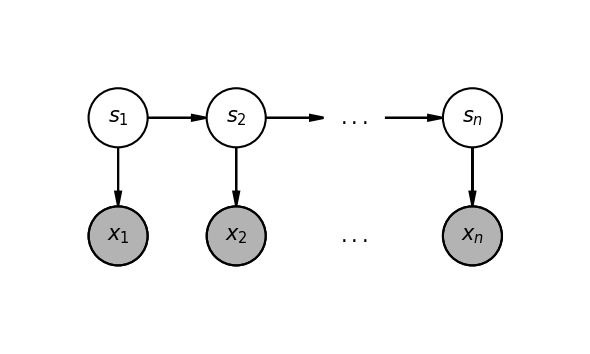
\includegraphics[width=0.5\paperwidth]{../HiddenMarkovModels/fig/HMM_DGM.png}
    \caption{The directed graphical model for an HMM.}
    \label{fig:HMM-DGM}
\end{figure}

We will probe HMMs in more detail over the course of the chapter, but for now let's consider their high-level properties.

\begin{mlcube}{Hidden Markov Models}
First, HMMs handle discrete states, and for the purpose of this text, we will only consider discrete-valued emissions as well. Second, since an HMM does not have access to the true states even at training time, it works on an unsupervised basis to approximate the hidden states. Finally, it's most common to probabilistically describe both the relationship between hidden states and observed emissions as well as the transitions between hidden states.
\begin{center}
    \begin{tabular}{c|c|c}
    \textit{\textbf{Domain}} & \textit{\textbf{Training}} & \textit{\textbf{Probabilistic}} \\
    \hline
    Discrete & Unsupervised & Yes \\
    \end{tabular}
\end{center}
\end{mlcube}
\readernote{Models that treat continuous state variables are commonly referred to as dynamical systems.}

\section{Applications}
Unsurprisingly, there are many applications for models like HMMs that explicitly account for time and unobserved states, especially those that relate to the physical world.
\begin{enumerate}
    \item Robot position when movements are non-deterministic and sensor readings are noisy.
    \item Speech recognition.
    \item Analyzing sequences that occur in the natural world, such as DNA.
\end{enumerate}

\section{HMM Data, Model, and Parameterization}
As explained above, HMMs model the state of an entity over time given some noisy observations, as shown in Figure \ref{fig:HMM-DGM}.

\subsection{HMM Data}
A complete data point for an HMM consists of the sequence of one-hot encoded states $\textbf{s}_1, ..., \textbf{s}_n$ as well as the corresponding sequence of observed emissions $\textbf{x}_1, ..., \textbf{x}_n$. Each state corresponds to one of $K$ possible options, meaning $\textbf{s}_t \in \mathbb{R}^K$, and each emission corresponds to one of $M$ possible options meaning $\textbf{x}_t \in \mathbb{R}^M$. Note that we don't have access to the complete data points, but only the observed emissions. It's our goal to infer the hidden states.
\readernote{In general the observed emissions don't have to be discrete, but for the sake of being explicit, we present the discrete interpretation here.}

Note that a single \textit{data point} consists of a sequence of $n$ emissions $\textbf{x}_1, ..., \textbf{x}_n$. A data set is said to have $N$ data points, meaning $N$ sequences where each sequence is composed of $n$ emissions. To summarize:
\begin{itemize}
	\item A data set consists of $N$ sequences.
	\item Each sequence is composed of $n$ observed emissions $\textbf{x}_1, ..., \textbf{x}_n$.
	\item It's our goal to infer the hidden states $\textbf{s}_1, ..., \textbf{s}_n$ for each sequence.
	\item Each emission $\textbf{x}_{t}$ takes on one of $M$ possible options.
	\item Each hidden state $\textbf{s}_{t}$ take on one of $K$ possible options.
\end{itemize}

\subsection{HMM Model Assumptions}
One goal of an HMM is to optimize the joint distribution over hidden states and observed emissions given by:
\begin{equation} \label{large-joint}
	p(\textbf{s}_1, ..., \textbf{s}_n, \textbf{x}_1, ..., \textbf{x}_n) = p(\textbf{s}_1, ..., \textbf{s}_n) p(\textbf{x}_1, ..., \textbf{x}_n | \textbf{s}_1, ..., \textbf{s}_n)
\end{equation}
It's not immediately obvious how we should go about optimizing the model for this complex joint distribution. Fortunately, HMMs make this problem easier via the following assumptions:
\begin{itemize}
    \item[1.] State $\textbf{s}_{t+1}$ depends only on the previous state $\textbf{s}_t$:
	    \begin{align*}
	    	p(\textbf{s}_{t+1} | \textbf{s}_{1}, ..., \textbf{s}_{t}, \textbf{x}_{1}, ..., \textbf{x}_{t}) = p(\textbf{s}_{t+1} | \textbf{s}_{t}) 
	    \end{align*}
    	This is the \textit{Markov Property}, and it means that given information at the previous time step, we can ignore all earlier time steps.
    \item[2.] At each time step $t$, the observed emission $\textbf{x}_t$ depends only on the current state $\textbf{s}_t$.
    	\begin{align*}
	    	p(\textbf{x}_{t} | \textbf{s}_{1}, ..., \textbf{s}_{t}, \textbf{x}_{1}, ..., \textbf{x}_{t-1}) = p(\textbf{x}_{t} | \textbf{s}_{t}) 
	    \end{align*}
\end{itemize}
\readernote{The Markovian assumption for transitions, as well as the fact that we don't observe the true states, gives rise to the \textit{Hidden Markov Model} name.}
Notice that these two assumptions allow us to factorize the large joint distribution given by Equation \ref{large-joint} as follows:
\begin{equation} \label{factorized-joint}
	p(\textbf{s}_1, ..., \textbf{s}_n) p(\textbf{x}_1, ..., \textbf{x}_n | \textbf{s}_1, ..., \textbf{s}_n) = p(\textbf{s}_1) \prod_{t=1}^{n-1} p(\textbf{s}_{t+1} | \textbf{s}_t) \prod_{t=1}^{n} p(\textbf{x}_t | \textbf{s}_t)
\end{equation}
This factorization will prove important for making HMM training and inference tractable.

\subsection{HMM Parameterization}
Now that we understand the form of the data as well as the modeling assumptions made by an HMM, we can specify the model parameterization explicitly. Referencing the factorized joint distribution from Equation \ref{factorized-joint}, it's clear that we will need three distinct sets of parameters.

\begin{itemize}
	\item[1.] One set of parameters is for the prior over our initial hidden state $p(\textbf{s}_1)$. It will be denoted $\boldsymbol{\theta} \in \mathbb{R}^{K}$, such that:
	\begin{align*}
		p(\textbf{s}_1 = k) = \theta_k
	\end{align*}

	\item[2.] Another set of parameters is for the transition probabilities between states $p(\textbf{s}_{t+1} | \textbf{s}_t)$. It will be denoted $\textbf{T} \in \mathbb{R}^{K \times K}$, such that:
	\begin{align*}
		p(\textbf{s}_{t+1} = j | \textbf{s}_t = i) = T_{i,j}
	\end{align*}
	where $T_{i,j}$ is the probability of transitioning from state $i$ to state $j$.

	\item[3.] Finally, we have a set of parameters for the conditional probability of the observed emission given the hidden state, meaning $p(\textbf{x}_t | \textbf{s}_t)$. It will be denoted $\boldsymbol{\pi} \in \mathbb{R}^{K \times M}$, such that:
	\begin{align*}
		p(\textbf{x}_t = m | \textbf{s} = k) = \pi_{k, m}
	\end{align*}
	A natural interpretation of the parameter matrix $\boldsymbol{\pi}$ is that each possible state (of which there are $K$ options) has an $M$-dimensional vector describing the probability of an emission given that state.
\end{itemize}

In sum, we have three sets of parameters $\boldsymbol{\theta} \in \mathbb{R}^{K}$, $\textbf{T} \in \mathbb{R}^{K \times K}$, and $\boldsymbol{\pi} \in \mathbb{R}^{K \times M}$ that we need to learn from our data set. Then, using this trained model, we will be able to perform several types of inference over our hidden states, which are detailed down below.

\section{EM for HMMs and the Forward-Backward Algorithm}
Recall the motivation for the Expectation-Maximization algorithm from the previous chapter: we had parameters we wished to optimize, but the presence of unobserved variables made direct optimization of those parameters intractable. We're faced with a similar problem in the context of HMMs.

Given a data set of observed emissions $\{ \textbf{x}^{i} \}_{i=1}^{N}$ where each data point $\textbf{x}^{i}$ represents the sequence $(\textbf{x}_{1}^{i}, ..., \textbf{x}_{n}^{i})$, our goal is to estimate the parameters $\boldsymbol{\theta}, \textbf{T}, \boldsymbol{\pi}$ described in the previous section. If we knew the hidden states, it would be possible for us to write the joint probability $p(\textbf{s}^{i}, \textbf{x}^{i})$ directly, and maximizing our parameters would be no issue. However, the true states are latent variables, and thus we would need to sum over their possible values, which is what makes the direct maximization of our parameters intractable.

Instead, we will use the Expectation-Maximization algorithm we developed in the previous chapter. This amounts to computing the expectation over our hidden states in the E-step, and then based on those fixed expectations, we can update our parameters via a maximization of the expected complete-data in the M-step. As usual, we perform these operations iteratively until convergence.

So far, there is no clear departure from the same exact EM algorithm we saw in the last chapter. However, before we go about detailing the E and M steps, we need to consider something known as the \textbf{Forward-Backward Algorithm}.

\subsection{Forward-Backward Algorithm}
Let's consider what would actually be required of us to perform the E-step for the hidden states of an HMM. To compute the expected value of state $\textbf{s}_t$ using the full joint distribution given by:
\begin{align*}
	p(\textbf{s}_1, ..., \textbf{s}_n, \textbf{x}_1, ..., \textbf{x}_n) = p(\textbf{s}_1) \prod_{t=1}^{n-1} p(\textbf{s}_{t+1} | \textbf{s}_t) \prod_{t=1}^{n} p(\textbf{x}_t | \textbf{s}_t)
\end{align*}
would require marginalizing over all the unobserved states other than $\textbf{s}_{t}$ as follows:
\begin{align*}
	\mathbb{E}[\textbf{s}_t | \textbf{s}_1, ..., \textbf{s}_{t-1}, \textbf{s}_{t + 1}, ..., \textbf{s}_n, \textbf{x}_1, ..., \textbf{x}_n] = p(\textbf{s}_t | \textbf{s}_1, ..., \textbf{s}_{t-1}, \textbf{s}_{t + 1}, ..., \textbf{s}_n, \textbf{x}_1, ..., \textbf{x}_n) &= \\
	\sum_{k^{(1)} \in K} ... \sum_{k^{(t-1)} \in K} \sum_{k^{(t+1)} \in K} ... \sum_{k^{(n)} \in K} p(\textbf{s}_t | \textbf{s}_1=k^{(1)}, ..., \textbf{s}_{t-1}=k^{(t-1)}, \textbf{s}_{t+1}=k^{(t+1)}, ..., \textbf{s}_n=k^{(n)}, \textbf{x}_1, ..., \textbf{x}_n)
\end{align*}

If we were to do this naively by marginalizing over all states at each time step, it would be a very expensive and wasteful computation. For example, computing the expected value of the state at time step 2 would require summing over all possible states for $\textbf{s}_1, \textbf{s}_3, ..., \textbf{s}_n$. Then, to get the expected value of the state at time step 3, we would need to sum over all possible states for $\textbf{s}_1, \textbf{s}_2, \textbf{s}_4, ..., \textbf{s}_n$. Notice that this approach duplicates a lot of work. Rather than performing these summations over and over again, we can instead memoize (or reuse) these summations using the Forward-Backward algorithm.

The Forward-Backward algorithm is an example of a \textit{message-passing} scheme, which means we compute information once and then pass it around our model in the form of compact, reusable messages. The goal is to avoid duplicating work, instead using the messages directly. If you've encounted dynamic programming before, the Forward-Backward Algorithm is an example. Ultimately, the purpose of the Foward-Backward algorithm is to make the expectation step over our HMM more efficient.

This algorithm passes messages, unsurprisingly, forwards and backwards through `time', meaning up and down the chain shown in the graphical model representation given by Figure \ref{fig:HMM-DGM}. The forward messages are defined at each state as $\alpha_t(\textbf{s}_t)$, while the backward messages are defined at each state as $\beta_t(\textbf{s}_t)$. Let's define these $\alpha$ and $\beta$ values explicitly.

The $\alpha_t$'s represent the joint probability of all our observed emissions from time $1,...,t$ as well as the state exactly at time $t$:
\begin{equation} \label{unfactorized-alphas}
	\alpha_t(\textbf{s}_t) = p(\textbf{x}_1, ..., \textbf{x}_t, \textbf{s}_t)
\end{equation}
Graphically, this means that the $\alpha_t$'s are capturing the portion of the DGM shown in Figure \ref{fig:HMM-DGM-alpha}.
\begin{figure}
    \centering
    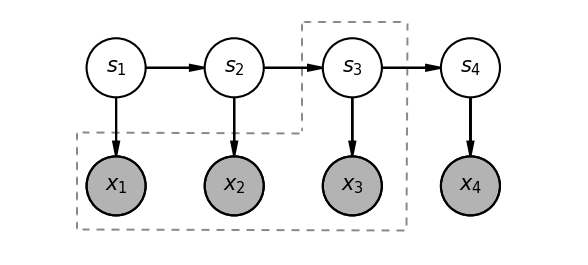
\includegraphics[width=0.5\paperwidth]{../HiddenMarkovModels/fig/HMM_DGM_alpha.png}
    \caption{$\alpha_t$'s capture the joint probability for the boxed portion of this DGM.}
    \label{fig:HMM-DGM-alpha}
\end{figure}

Note that Equation \ref{unfactorized-alphas} is an unfactorized joint probability over observed emissions and a hidden state. We can factorize this joint probability using what we know about the conditional independence properties of HMMs as follows:
\begin{align} \label{factorized-alphas}
	\alpha_t(\textbf{s}_t) &= p(\textbf{x}_1, ..., \textbf{x}_t, \textbf{s}_t) \\
	&= p(\textbf{x}_t | \textbf{s}_t) \sum_{\textbf{s}_{t-1}} p(\textbf{s}_t | \textbf{s}_{t-1}) p(\textbf{x}_1, ..., \textbf{x}_{t-1}, \textbf{s}_{t-1}) \\
	&= p(\textbf{x}_t | \textbf{s}_t) \sum_{\textbf{s}_{t-1}} p(\textbf{s}_t | \textbf{s}_{t-1}) \alpha_{t-1}(\textbf{s}_{t-1})
\end{align}
Pay careful attention to the last line of Equation \ref{factorized-alphas}. Notice that our expression for $\alpha_t(\textbf{s}_t)$ actually includes the expression for $\alpha_{t-1}(\textbf{s}_{t-1})$, which is the $\alpha$ from the previous time step. This is significant because it means we can define our messages \textit{recursively}. After we've computed the $\alpha$'s at one time step, instead of having to recompute those values to get the alphas at the next time step, we can simply \textit{pass} them forwards along the chain. In other words, we compute the $\alpha$ at state $\textbf{s}_1$, then pass that message along to compute the $\alpha$ at state $\textbf{s}_2$, on and on until we've reached the end of the chain and have all the $\alpha$'s in hand.
\readernote{These $\alpha$ values will be useful when performing the expectation step during training, as well as for general inference once we've finished training our HMM.}

At this point, we've now handled the forward messages, which send information from the beginning to the end of the chain. We also need to send information from the end of the chain back to the beginning, which constitutes the backwards portion of the algorithm. This is where we will compute our $\beta$ values.

The $\beta_t$'s represent the joint probability over all the observed emissions from time $t+1, ..., n$ conditioned on the state at time $t$:
\begin{equation} \label{unfactorized-betas}
	\beta_t(\textbf{s}_t) = p(\textbf{x}_{t+1}, ..., \textbf{x}_n | \textbf{s}_t)
\end{equation}
Graphically, this means that the $\beta_t$'s are capturing the portion of the DGM shown in Figure \ref{fig:HMM-DGM-beta}.
\begin{figure}
    \centering
    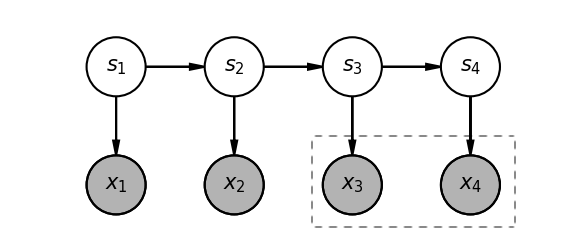
\includegraphics[width=0.5\paperwidth]{../HiddenMarkovModels/fig/HMM_DGM_beta.png}
    \caption{$\beta_t$'s capture the joint probability for the boxed portion of this DGM.}
    \label{fig:HMM-DGM-beta}
\end{figure}

We can factorize Equation \ref{unfactorized-betas} in a similar way to how we factorized the distribution described by the $\alpha$'s:
\begin{align} \label{factorized-betas}
	\beta_t(\textbf{s}_t) &= p(\textbf{x}_{t+1}, ..., \textbf{x}_n | \textbf{s}_t) \\
	&= \sum_{\textbf{s}_{t+1}} p(\textbf{s}_{t+1} | \textbf{s}_t) p(\textbf{x}_{t+1}, ..., \textbf{x}_n | \textbf{s}_{t+1}) \\
	&= \sum_{\textbf{s}_{t+1}} p(\textbf{s}_{t+1} | \textbf{s}_t) p(\textbf{x}_{t+1} | \textbf{s}_{t+1}) p(\textbf{x}_{t+2}, ..., \textbf{x}_n | \textbf{s}_{t+1}) \\
	&= \sum_{\textbf{s}_{t+1}} p(\textbf{s}_{t+1} | \textbf{s}_t) p(\textbf{x}_{t+1} | \textbf{s}_{t+1}) \beta_{t+1}(\textbf{s}_{t+1})
\end{align}
Again, as we saw with our calculation of the $\alpha$'s, we have our $\beta$'s defined recursively. Once again, this means that we can propagate messages efficiently. In this case, we start at the end of the chain, and compute our $\beta$'s for each state by passing messages back toward the front.

To summarize, the Forward-Backward algorithm is an optimization that will boost efficiency for the EM algorithm as well as for inference over a trained HMM. We calculate the $\alpha$ and $\beta$ values as follows:
\begin{align*}
	\alpha_t(\textbf{s}_t) &=
	\begin{cases} 
      p(\textbf{x}_t | \textbf{s}_t) \sum_{\textbf{s}_{t-1}} p(\textbf{s}_t | \textbf{s}_{t-1}) \alpha_{t-1}(\textbf{s}_{t-1}) & 1 < t \leq n \\
      p(\textbf{x}_1 | \textbf{s}_{1}) p(\textbf{s}_1) & \text{otherwise} \\
   \end{cases} \\
   \beta_t(\textbf{s}_t) &=
   \begin{cases} 
      \sum_{\textbf{s}_{t+1}} p(\textbf{s}_{t+1} | \textbf{s}_t) p(\textbf{x}_{t+1} | \textbf{s}_{t+1}) \beta_{t+1}(\textbf{s}_{t+1}) & 1 \leq t < n \\
      1 & \text{otherwise} \\
   \end{cases}
\end{align*}
\readernote{Notice that the base case for the $\beta$'s is 1. This is just a quirk of our indexing, and it ensures we have valid messages when we pass messages back from the final state $\textbf{s}_n$.}

\subsection{Using $\alpha$'s and $\beta$'s for Training and Inference}
Now that we know how to compute these $\alpha$ and $\beta$ values, we need to consider how we actually use them for training and inference within our HMM setup. Indeed, it's not immediately clear how the distributions defined by the $\alpha$'s and $\beta$'s are useful.

Let's begin by assuming we randomly initialized our model parameters $\boldsymbol{\theta}, \textbf{T}, \boldsymbol{\pi}$, and then used these to compute all the $\alpha$ and $\beta$ values by passing messages up and down the chain (using the recurrences defined at the end of the last section). We now have $\alpha$ and $\beta$ values defined at every time step in our HMM. Consider the product of the $\alpha$ and $\beta$ value at a specific time $t$:
\begin{align*}
	\alpha_t(\textbf{s}_t) \beta_t(\textbf{s}_t) = p(\textbf{x}_1, ..., \textbf{x}_t, \textbf{s}_t) p(\textbf{x}_{t+1}, ..., \textbf{x}_n | \textbf{s}_t) = p(\textbf{x}_1, ..., \textbf{x}_n, \textbf{s}_t)
\end{align*}
which is just the joint distribution over all our observed emissions and the state at time $t$. Using this as a building block, there are many distributions over the variables in our HMM that we can evaluate. For example, we might like to evaluate the joint distribution over our observed emissions.

\subsubsection{Joint Distribution Over Emissions}
\begin{equation} \label{joint-fn}
	p(\textbf{x}_1, ..., \textbf{x}_n) = \sum_{\textbf{s}_t \in K} \alpha_t(\textbf{s}_t) \beta_t(\textbf{s}_t)
\end{equation}
where we can sum over the possible state values at any time step $1,...,n$.

Another useful distribution is that of the state at time $t$ given all the observed emissions. This has the name \textit{smoothing}, which in some contexts means updating our beliefs given observed evidence.

\subsubsection{Smoothing}
\begin{equation} \label{smoothing-fn}
	p(\textbf{s}_t | \textbf{x}_1, ..., \textbf{x}_n) \propto p(\textbf{x}_1, ..., \textbf{x}_t, \textbf{s}_t) = \alpha_t(\textbf{s}_t) \beta_t(\textbf{s}_t)
\end{equation}
Notice that the proportionality of the smoothing operation means we can normalize to recover probabilities by taking the softmax over the possible values for the state $\textbf{s}_t$. \newline \newline
Another common task is predicting the value of the next emission given the previous emissions.

\subsubsection{Prediction}
\begin{equation} \label{prediction-fn}
	p(\textbf{x}_{n+1} | \textbf{x}_1, ..., \textbf{x}_n)
\end{equation}
To compute this we can sum over the final state $\textbf{s}_n$ as well as the next state $\textbf{s}_{n+1}$ as follows:
\begin{align}
	p(\textbf{x}_{n+1} | \textbf{x}_1, ..., \textbf{x}_n) &\propto \sum_{\textbf{s}_n} \sum_{\textbf{s}_{n+1}} p(\textbf{x}_1, ..., \textbf{x}_n, \textbf{s}_n) p(\textbf{s}_{n+1} | \textbf{s}_n) p(\textbf{x}_{n+1} | \textbf{s}_{n+1}) \\
	&\propto \sum_{\textbf{s}_n} \sum_{\textbf{s}_{n+1}} \alpha_{n}(\textbf{s}_n) p(\textbf{s}_{n+1} | \textbf{s}_n) p(\textbf{x}_{n+1} | \textbf{s}_{n+1})
\end{align}
Again, we recover a proportional result from this operation. We can use the softmax over the emissions states to normalize.

Finally, we may wish to approximate the transition probabilities between states $\textbf{s}_t$ and $\textbf{s}_{t+1}$ given all the observed evidence.

\subsubsection{Transition}
\begin{align} \label{transition-fn}
	p(\textbf{s}_{t}, \textbf{s}_{t+1} | \textbf{x}_1, ..., \textbf{x}_n) &\propto p(\textbf{x}_1, ..., \textbf{x}_t, \textbf{s}_t) p(\textbf{s}_{t+1} | \textbf{s}_{t}) p(\textbf{x}_{t+1} | \textbf{s}_{t+1}) p(\textbf{x}_{t+2}, ..., \textbf{x}_{n} | \textbf{s}_{t+1}) \\
	&\propto \alpha_t(\textbf{s}_t) p(\textbf{s}_{t+1} | \textbf{s}_{t}) p(\textbf{x}_{t+1} | \textbf{s}_{t+1}) \beta_{t+1}(\textbf{s}_{t+1}) \\
\end{align}
where we again have proportionality results that can be normalized if necessary.

Now that we understand how exactly $\alpha$ and $\beta$ values can be used to evaluate different distributions of interest for an HMM, we can finally turn to using EM to optimize the parameters of our model.

\subsection{E-Step}
Recall that the goal of the expectation step is to compute the expected values of the hidden variables in our model given a fixed set of parameters. Our parameters are $\boldsymbol{\theta}, \textbf{T}, \boldsymbol{\pi}$. Note that the $\alpha$ and $\beta$ values described in the previous section are exact functions of these parameters, so at the start of the E-step, we should compute them using the efficient Forward-Backward algorithm. It will become clear why we need the $\alpha$ and $\beta$ values as we explain the E-step.

Under the HMM setup, our hidden variables are the states $\textbf{s}_1, ..., \textbf{s}_n$. Since we have $N$ emission sequences $\textbf{x}^i = (\textbf{x}_1^i, ..., \textbf{x}_n^i) \quad \forall i \in N$ in our data set, we will end up with $N$ expected sequences over our hidden states:
\begin{align*}
	\textbf{q}^i = \mathbb{E}[(\textbf{s}_1^i, ..., \textbf{s}_n^i) | (\textbf{x}_1^i, ..., \textbf{x}_n^i)] \quad \forall i \in N
\end{align*}
Where $\textbf{q}^i \in \mathbb{R}^{n \times K}$, corresponding to the expectation of each state at each time step. Let's consider $q_{t, k}^i$ which is the expectation over a single state value $k$ at a single point in time $t$. We can write this as:
\begin{align}
	q_{t, k}^i &= \mathbb{E}[s_{t, k}^i | (\textbf{x}_1^i, ..., \textbf{x}_n^i)] \\
	&= p(\textbf{s}_{t}^i = k | (\textbf{x}_1^i, ..., \textbf{x}_n^i))
\end{align}
This calculates the probability of a single state given all of our observed emissions for a single data point. This is exactly the smoothing operation described in the previous section! That is why we calculated our $\alpha$ and $\beta$ values at the beginning of the E-step using our fixed parameters, because we can now easily use the smoothing operation given by Equation \ref{smoothing-fn} to compute our $\textbf{q}_t^i$ values.

Ordinarily, we'd be done with the E-step after computing the expectations of our hidden variables, but under the HMM setup, we need to take one more expectation before moving on to the M-step. Recall that we have transition probabilities between our hidden states given by the parameter matrix $\textbf{T}$. Because these are transitions between latent variables, we also need to compute the expectation over the joint distribution between pairs of latent variables next to each other in time, which we will denote $\textbf{Q}_{t, t+1}^i \in \mathbb{R}^{K \times K}$. Formally:
\begin{align}
	\textbf{Q}_{t, t+1}^i = \mathbb{E}[\textbf{s}_t^i, \textbf{s}_{t+1}^i | (\textbf{x}_1^i, ..., \textbf{x}_n^i)]
\end{align}
Let's consider $Q_{t, t+1, k, l}^i$ which is the transition from state $k$ at time step $t$ to state $l$ at time step $t+1$:
\begin{align}
	Q_{t, t+1, k, l}^i &= \mathbb{E}[\textbf{s}_{t}^i = k, \textbf{s}_{t+1}^i = l | (\textbf{x}_1^i, ..., \textbf{x}_n^i)] \\
	&= p(\textbf{s}_{t}^i = k, \textbf{s}_{t+1}^i = l | (\textbf{x}_1^i, ..., \textbf{x}_n^i)) \\
\end{align}
This is calculating the probability of a specific latent variable transition at a specific time step, which is exactly the transition operation described in the previous section. We can directly use our $\alpha$ and $\beta$ values in the transition operation given by Equation \ref{transition-fn}.

With our $\textbf{q}^i$ and $\textbf{Q}^i$ values as expectations over the hidden states and hidden joint states respectively (with the current setting of our parameters fixed), we are ready to move on to the maximization step.

\subsection{M-Step}
The M-step mirrors what we saw in the previous chapter. In the E-step we calculated expectations over our hidden variables, which allows us to set up our expected complete-data log likelihood for a single data point:
\begin{align*}
	\mathbb{E}_{\textbf{q}, \textbf{Q}}[\log p(\textbf{x}^i, \textbf{s}^i; \boldsymbol{\theta}, \textbf{T}, \boldsymbol{\pi})] &= \mathbb{E}_{\textbf{q}, \textbf{Q}} \bigg[ \log p(\textbf{x}^i | \textbf{s}^i; \boldsymbol{\pi}) + \log p(\textbf{s}^i; \boldsymbol{\theta}, \textbf{T}) \bigg] \\
	&= \sum_{t=1}^{n} \sum_{k=1}^{K} q_{t, k}^{i} \sum_{m=1}^{M} \log \pi_{k, x_{t, m}^i} + \sum_{k=1}^{K} q_{k}^{i} \log \theta_k + \sum_{t=1}^{n-1} \sum_{k=1}^{K} \sum_{l=1}^{K} Q_{t, t+1, k, l}^{i} \log T_{k, l} \\
\end{align*}
Applying the appropriate Lagrange multipliers and maximizing with respect to each of the parameters of interest, we recover the following update equations:
\begin{align}
	\theta_k &= \frac{\sum_{i=1}^{N} q_{1, k}^i}{N}
\end{align}
\begin{align}
	T_{k, l} &= \frac{\sum_{i=1}^{N} \sum_{t=1}^{n-1} Q_{t, t+1, k, l}^i}{\sum_{i=1}^{N} \sum_{t=1}^{n-1} q_{t, k}^i}
\end{align}
\begin{align}
	\pi_{k, m} &= \frac{\sum_{i=1}^{N} \sum_{t=1}^{n} q_{t, k}^i x_{t, m}^i}{\sum_{i=1}^{N} \sum_{t=1}^{n} q_{t, k}^i}
\end{align}
After updating our parameter matrices $\boldsymbol{\theta}, \textbf{T}, \boldsymbol{\pi}$, we switch back to the E-step, continuing in this way until convergence of our parameters.

\subsection{From HMM Training to Inference}
In the preceding sections, we described the process for training an HMM. In doing so, we've actually built up all the machinery needed to perform inference on our trained HMM for free. Specifically, we've described four types of queries we can execute over a trained HMM:
\begin{itemize}
	\item Joint Estimation
	\item Prediction
	\item Smoothing
	\item Transition
\end{itemize}
We analyzed these already because we needed them to train the HMM, but once we've completed training, we can use our optimized parameters along with the $\alpha$ and $\beta$ values that we compute with the Forward-Backward algorithm to query our HMM.

\section{Conclusion}
The Hidden Markov Model is a type of latent variable model motivated by the combination of time series and discrete state space data. We relied on the Expectation-Maximization algorithm described in the previous chapter, and developed the efficient Forward-Backward algorithm to make both training and inference feasible for HMMs. Many of the ideas developed in this chapter will offer good intuition for dynamical systems and other time series models.